\documentclass[../main.tex]{subfiles}
\begin{document}
\chapter{Immagini di batteri ESKAPE}

\section{SSNOMBACTER}

Le immagini elaborate in questa tesi sono prese dal dataset di SSNOMBACTER, pubblicato su GigaScience nel 2020. Questo dataset comprende oltre 4000 immagini di 15 diverse specie batteriche generate da un microscopio \acrshort{ssnom} con lo scopo di promuovere applicazioni nella \Gls{microbiologia} e aumentare la popolarità di questa tecnica.\cite{ssnombacter}

Queste immagini sono state generate da un microscopio NeaSNOM in modalità a contatto intermittente usando un laser con una lunghezza d'onda di $1,550$ \micro m ($6,451.61$ \gls{cm-1}) e un cantilever placcato in oro con un raggio alla punta minore di $35$ nm, una frequenza di risonanza di 65kHz e una costante elastica di $0.5\ N/m$. (HQ:NSC19/Cr-Au)\cite{micromasch}

Per ogni specie batterica sono state generate almeno 3 immagini su regioni diverse con un campo visivo di 10 \micro m × 10 \micro m, e almeno una con un campo visivo ingrandito, tra 2 \micro m × 2 \micro m e 4 \micro m × 4 \micro m, in base alle dimensioni della specie selezionata. Sono state generate sia immagini \acrshort{snom} che \acrshort{afm} della stessa regione esaminata per avere una caratterizzazione più completa e dettagliata delle specie batteriche, potendo infatti ricavare sia proprietà ottiche che topologiche o morfologiche usando degli appositi algoritmi di elaborazione. 

Le immagini \acrshort{ssnom} provvedono l'ampiezza e la fase dello spettro, da cui è possibile ricavare le proprietà dielettriche del campione, mentre le immagini \acrshort{afm} ne provvedono la topografia e le proprietà viscoelastiche. L'oggetto di questa tesi è comparare i due tipi di immagini e verificare quali caratteristiche morfologiche possono essere estratte da esse.

I dati delle scansioni sono disponibili sia in formato \textit{Gwyddion Simple Fields}\cite{gwyddion} (\texttt{.gsf})\footnote{La specifica del file è disponibile online\\URL: \url{https://gwyddion.net/documentation/user-guide-en/gsf.html}}, in cui sono disponibili i valori reali delle scansioni, sia come immagini \texttt{.tiff} con valori interi compresi tra $0$ e $255$. Ogni scansione è locata in una cartella a sé e i nomi dei file seguono questo modello:

\begin{center}
[ceppo batterico] [numero FOV] [abbreviazione tipo immagine]
\end{center}

Ogni scansione è inoltre provvista di un file \texttt{.txt} con i parametri di acquisizione usati, come il tempo di integrazione, la frequenza di oscillazione della punta, i parametri del controllore \acrshort{pid}, la sorgente laser e la frequenza di modulazione.

\begin{table}[h!t]
\centering
\begin{tabular}{l|l}
	Abbr. & Descrizione\\
	\hline\hline
	M0A & AFM --- Errore topografia\\
	M1A & AFM --- Errore topografia; 1\textsuperscript{a} armonica\\
	M2A & AFM --- Errore topografia; 2\textsuperscript{a} armonica\\
	M3A & AFM --- Errore topografia; 3\textsuperscript{a} armonica\\
	M4A & AFM --- Errore topografia; 4\textsuperscript{a} armonica\\
	M5A & AFM --- Errore topografia; 5\textsuperscript{a} armonica\\
	M1P & AFM --- Fase topografia; 1\textsuperscript{a} armonica\\
	M2P & AFM --- Fase topografia; 2\textsuperscript{a} armonica\\
	M3P & AFM --- Fase topografia; 3\textsuperscript{a} armonica\\
	M4P & AFM --- Fase topografia; 4\textsuperscript{a} armonica\\
	M5P & AFM --- Fase topografia; 5\textsuperscript{a} armonica\\
	O0A & SNOM --- Ampiezza\\
	O1A & SNOM --- Ampiezza; 1\textsuperscript{a} armonica\\
	O2A & SNOM --- Ampiezza; 2\textsuperscript{a} armonica\\
	O3A & SNOM --- Ampiezza; 3\textsuperscript{a} armonica\\
	O4A & SNOM --- Ampiezza; 4\textsuperscript{a} armonica\\
	O5A & SNOM --- Ampiezza; 5\textsuperscript{a} armonica\\
	O1P & SNOM --- Fase; 1\textsuperscript{a} armonica\\
	O2P & SNOM --- Fase; 2\textsuperscript{a} armonica\\
	O3P & SNOM --- Fase; 3\textsuperscript{a} armonica\\
	O4P & SNOM --- Fase; 4\textsuperscript{a} armonica\\
	O5P & SNOM --- Fase; 5\textsuperscript{a} armonica\\
	Z & AFM --- Topografia
\end{tabular}
\caption{Tipi di immagini presenti nel dataset}
\end{table}

\section{Batteri}

In \Gls{microbiologia}, i batteri sono un regno (\textit{Bacteria}) comprendente organismi unicellulari procarioti, le cui dimensioni possono variare tra circa $0.2$ \micro m e $30$ \micro m.\cite{goker_2024} I batteri sono stati tra le prime forme di vita ad apparire sulla Terra e sono presenti nella maggior parte dei suoi habitat. Alcuni batteri sono innocui, o perfino utili\cite{mccutcheon_2021}, per gli altri esseri viventi ma altre specie possono vivere a spese loro e arrecargli danni, anche gravi.\cite{johnson_2018}
\medskip

\begin{figure}[h]
	\centering
	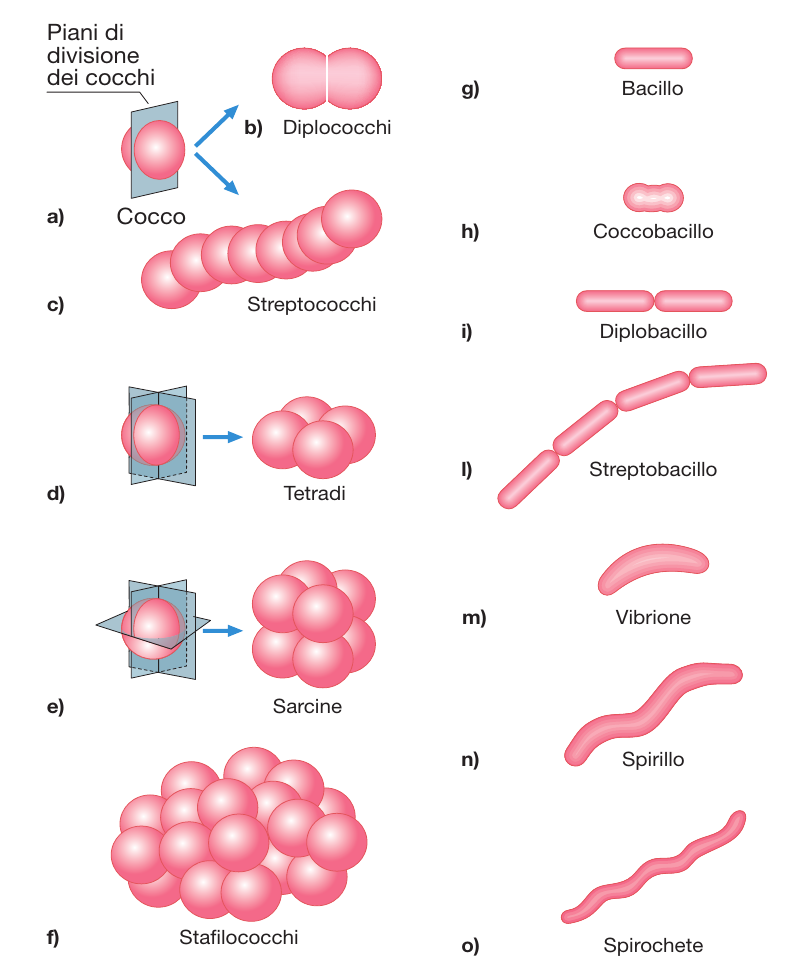
\includegraphics[keepaspectratio, width=0.95\linewidth]{images/batteri_morfologia.png}
	\caption[Tipiche forme di aggregati batterici]{
		Tipiche forme di aggregati batterici \cite{deho_galli_2020}}
	\label{fig:bacteria_morphology}
\end{figure}

\subsection{Morfologia}

Le dimensioni ridotte dei batteri fa sì che il loro rapporto superficie/volume sia in genere molto più elevato di quello delle cellule eucariote (dimensioni lineari tipiche nell'ordine delle decine di \micro m), con ovvie conseguenze sulla velocità con cui avvengono gli scambi molecolari tra cellula e ambiente, il trasporto di nutrienti, la crescita, la divisione cellulare e, di conseguenza, anche l'evoluzione. \cite{deho_galli_2020}

Essendo organismi unicellulari, i batteri presentano una limitata varietà di forme, che si possono raggruppare in questi gruppi: \textbf{Cocchi}, \textbf{Bacilli}, \textbf{Coccobacilli}, \textbf{Spirali}, \textbf{Elicoidali}.

Un \textbf{bacillo}, anche chiamato \textit{batterio bacilliforme}, è un microrganismo a forma di bastoncino. Esiste anche un genere tassonomico chiamato \textit{Bacillus} ma i bacilli si possono trovare anche in molti altri gruppi batterici. I bacilli di solito si dividono sullo stesso piano e sono solitari, ma possono anche combinarsi in agglomerati:

\begin{itemize}
	\itemsep0em 
	\item I diplobacilli sono coppie di bacilli legate sul lato corto.
	\item Gli streptobacilli sono catene di bacilli.
	\item I coccobacilli hanno una forma più ovale, simile ai cocchi.
\end{itemize}

Un \textbf{cocco}, anche chiamato \textit{batterio coccoide}, è un microrganismo la cui forma è pressoché sferica. I batteri coccoidi si presentano spesso in disposizioni caratteristiche e anche queste forme hanno nomi specifici: \cite{zapun_2008}

\begin{itemize}
	\itemsep0em 
	\item I diplococchi sono coppie di cocchi.
	\item Gli streptococchi sono catene di cocchi (come \textit{Streptococcus pyogenes}).
	\item Gli stafilococchi sono gruppi irregolari di cocchi (com \textit{Staphylococcus aureus}).
	\item I tetradi sono cluster di quattro cocchi disposti all'interno dello stesso piano (come \textit{Micrococcus sp.}).
	\item I Sarcina sono cluster di otto cocchi a disposizione cuboidale (come \textit{Sarcina Ventriculi}).
\end{itemize}

Contrariamente a molti batteri bacilliformi, la maggior parte dei batteri cocchi non ha flagelli e non possono muoversi autonomamente.\cite{levinson_2018}

\subsection{Parete cellulare}

La morfologia batterica è determinata da una parete costituita da una macromolecola gigante di \textbf{peptidoglicano}, un polisaccaride complesso, che avvolge tutta la cellula. La parte più interna di questa struttura è la membrana plasmatica ed è presente in tutte le cellule. La parete invece può assumere strutture diverse, che definiscono la Gram-positività di un batterio, o anche avere appendici sulla superficie (come dei flagelli) e ulteriori strati. Queste strutture di superficie conferiscono loro ulteriori proprietà per interagire con ambienti complessi, come ad esempio quelli costituiti da altre cellule, incluse quelle di ospiti animali, vegetali o microbici con cui il microrganismo può instaurare relazioni di simbiosi o di parassitismo.\cite{smith_1977}

La classificazione dei batteri secondo la colorazione di Gram prende il nome dal suo autore \textit{Hans Christian Gram}, che sviluppò il metodo nel 1884. Questo metodo consente di distinguere tra batteri Gram-positivi e Gram-negativi sulla base della colorazione differenziale tra un complesso cristal violetto-iodio (CV-I) e una controcolorazione di safranina. Le pareti cellulari degli organismi Gram-positivi mantengono questo complesso dopo il trattamento con alcol e sembrano viola, mentre gli organismi Gram-negativi decolorano a seguito di tale trattamento e sembrano rosa. Questo metodo è ancora oggi utile per valutare la contaminazione batterica dei campioni di coltura tissutale o per esaminare lo stato della colorazione di Gram e le caratteristiche morfologiche dei batteri isolati da colture batteriche miste o isolate.\cite{coico_2005}

\begin{figure}[h]
	\begin{subfigure}{0.5\linewidth}
		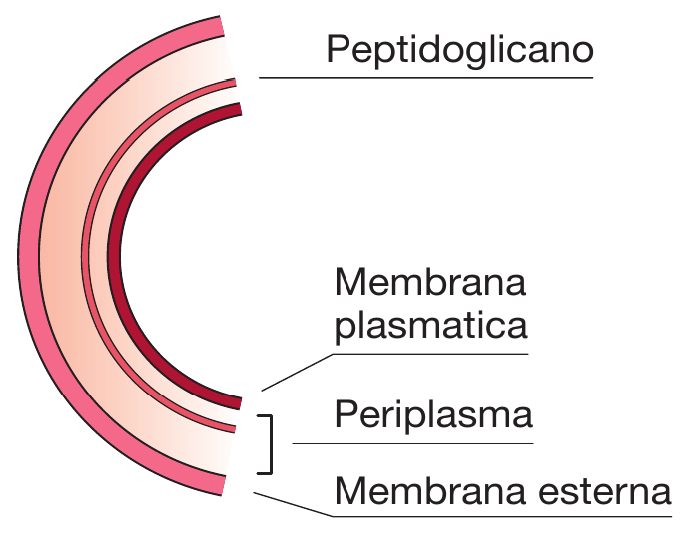
\includegraphics[keepaspectratio, width=\linewidth]{images/batterio_parete_neg.png}
		\caption{Gram negativi}
	\end{subfigure}
		\begin{subfigure}{0.5\linewidth}
		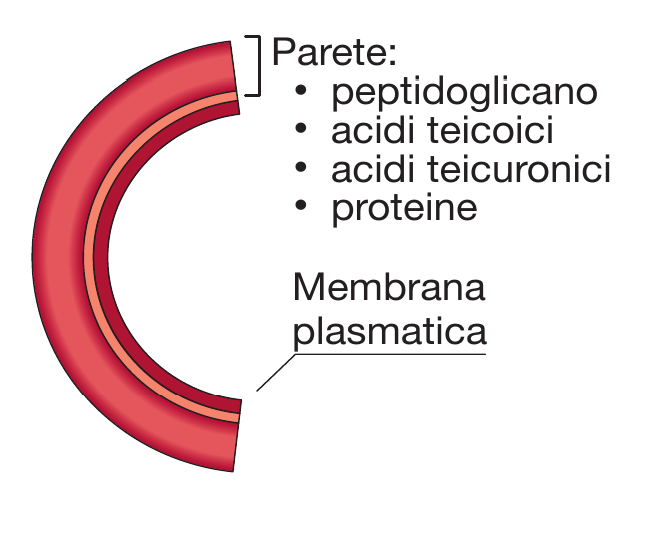
\includegraphics[keepaspectratio, width=\linewidth]{images/batterio_parete_pos.png}
		\caption{Gram positivi}
	\end{subfigure}
	\caption[Rappresentazione schematica del rivestimento cellulare]{
		Rappresentazione schematica del rivestimento cellulare \cite{deho_galli_2020}}
	\label{fig:bacteria_wall}
\end{figure}

\subsection{Fattori di virulenza}

Comprendere i fattori di virulenza e patogenicità dei batteri è importante perché rappresentano dei potenziali obiettivi per il rilevamento degli agenti patogeni. Nel linguaggio comune questi termini sono spesso confusi o usati intercambiabilmente ma, per definizione, la patogenicità misura l'abilità di un organismo ad indurre una malattia, mentre la virulenza misura la gravità relativa della malattia.\cite{watson_1949} Misurare la virulenza di un organismo è molto complesso a causa della moltitudine di variabili che dipendono sia dal patogeno che dall'ospite e dalla loro interazione.\cite{casadevall_2001}

Considerando i problemi sulla definizione della virulenza, anche i fattori di virulenza sono stati difficili da caratterizzare. Pertanto è importante comprendere i fattori di virulenza, poiché questi possono spesso essere utilizzati per rilevare i microrganismi patogeni. I fattori di virulenza tradizionali includono fattori che possono essere di aiuto in diverse fasi dell'infezione: \cite{love_2008}

\begin{itemize}
	\itemsep0em 
	\item Adesione alla cellula ospite
	\item Ingresso nella cellula ospite
	\item Elusione del rilevamento da parte del sistema immunitario dell'ospite
	\item Replicazione intracellulare o extracellulare e inibizione della fagocitosi
\end{itemize}

Questi fattori possono essere sia necessari, ovvero che la presenza o meno del suo gene produttore influenzi la patogenicità della specie, oppure contributivi, cioè che alterano la gravità della malattia. Il consenso generale è che, indipendentemente dalla funzione di un prodotto genico, se la sua espressione porta a un danno alla cellula ospite, allora si tratta di un fattore di virulenza.\cite{casadevall_1999}

\subsection{Adesione}

L'adesione ad una cellula ospite, o una matrice extracellulare, è un fattore importante per stabilire l'abilità di un microrganismo a provocare danni all'ospite. Questa adesione è mediata da molecole specifiche chiamate adesine, che possono essere proteiche e si suddividono principalmente in due categorie: adesine afimbriali (non filamentose) e fimbrie o pili, strutture filamentose presenti soprattutto nei batteri Gram-negativi (rari nei Gram-positivi).

I pili si osservano al microscopio elettronico come strutture simili a peli e sono fondamentali per l'adesione in batteri patogeni (come \textit{Vibrio cholerae}), che è influenzata in particolar modo dalle proteine sull'estremità dei pili.\cite{fallman_2005} Altri batteri possiedono più geni per la produzione di fimbrie, e solo la rimozione combinata di tutti questi operoni ha dimostrato di ridurre significativamente la virulenza, suggerendo che i fattori di adesione possono compensarsi a vicenda.

Un'altra forma di adesione piliforme sono i curli, presenti in ceppi di \textit{Escherichia coli} e \textit{Salmonella}.\cite{kenny_1997} Queste strutture sottili e irregolari sono altamente stabili e si legano a proteine dell'ospite come plasminogeno e fibronectina. Anche se i meccanismi di assemblaggio delle fimbrie variano, condividono caratteristiche strutturali comuni.\cite{soto_1999}\smallskip

\begin{figure}[h]
	\begin{subfigure}{0.5\linewidth}
		\centering
		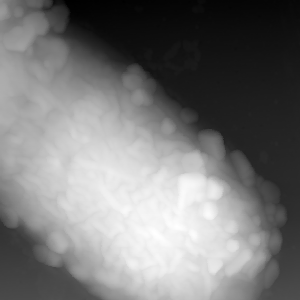
\includegraphics[keepaspectratio, width=0.65\linewidth]{images/ecoli_afm.png}
		\caption{Topografia AFM}
	\end{subfigure}
	\begin{subfigure}{0.5\linewidth}
		\centering
		
\includegraphics[keepaspectratio, width=0.65\linewidth]{images/ecoli_snom.png}
		\caption{Ampiezza SNOM --- $2^{a}$ armonica}
	\end{subfigure}
	\caption[Un esemplare di \textit{Escherichia Coli} visto al microscopio s-SNOM]{
		\begin{tabular}[t]{ @{} l @{} }
			Un esemplare di \textit{Escherichia Coli} visto al microscopio \acrshort{ssnom} \cite{ssnombacter_data}\\
			Si possono apprezzare le strutture sulla parete cellulare
		\end{tabular}}
	\label{fig:ecoli}
\end{figure}

Molte adesine, oltre a favorire l'adesione, giocano un ruolo nella fuga dal sistema immunitario dell'ospite. Sia i batteri Gram-negativi che quelli Gram-positivi esprimono una vasta gamma di adesine, che si legano a un ampio numero di bersagli cellulari, come immunoglobuline, glicoproteine, glicolipidi e proteine della matrice extracellulare.\cite{finlay_1997}

In conclusione, l'adesione dei batteri all'ospite è un processo complesso, che coinvolge numerosi tipi di adesine e meccanismi fondamentali non solo per l'inizio dell'infezione, ma anche per la sopravvivenza e la diffusione del patogeno.

\subsection{Plasticità morfologica}

Alcune specie di batteri posseggono, inoltre, la capacità di modificare la loro forma e dimensioni in risposta a condizioni ambientali avverse, chiamata plasticità morfologica. Questa adattabilità consente ai batteri di sopravvivere e proliferare in ambienti ostili, come quelli caratterizzati da stress nutrizionali, esposizione a antibiotici o attacchi del sistema immunitario dell'ospite. Questa strategia è fondamentale nella sopravvivenza dei batteri, permettendo loro di adattarsi e persistere in condizioni avverse per poi ritornare alla forma originale una volta ripristinate le condizioni favorevoli.\cite{justice_2008}\bigskip

\subsection{Gruppo ESKAPE}

Tra i ceppi batterici esaminati in SSNOMBACTER sono presenti alcuni ceppi patogeni altamente virulenti e resistenti a terapie antibiotiche. Questo gruppo di sei ceppi prende il nome di \textbf{ESKAPE}, formato dalle lettere iniziali di:

\begin{itemize}
	\itemsep0em
	\item \textit{Enterococcus faecium}
	\item \textit{Staphylococcus aureus}
	\item \textit{Klebsiella pneumoniae}
	\item \textit{Acinetobacter baumannii}
	\item \textit{Pseudomonas aeruginosa}
	\item \textit{Enterobacter spp}
\end{itemize}

\begin{table}[h!t]
	\centering
	\resizebox{\columnwidth}{!}{%
		\begin{tabular}{|l c l l|}
			\hline
			Ceppo batterico & Gram & Origine & Regioni acquisite \\
			\hline\hline
			\begin{tabular}{@{}l@{}}
				Achromobacter xylosoxidans\\ATCC 27061 (DSMZ 2402)T
			\end{tabular}	& --- &	Yabuuchi and Oyama 1971 \cite{yabuuchi_1971} &
			\begin{tabular}{@{}l@{}}
				3 × (10 \micro m × 10 \micro m)\\1 × (2 \micro m × 2 \micro m)
			\end{tabular}\\\hline
			\begin{tabular}{@{}l@{}}
				Acinetobacter baumannii\\ATCC 17978
			\end{tabular}	& --- & Sahm et al. 1989 \cite{sahm_1989} & 
			\begin{tabular}{@{}l@{}}
				4 × (10 \micro m × 10 \micro m)\\1 × (2 \micro m × 2 \micro m)
			\end{tabular}\\\hline
			\begin{tabular}{@{}l@{}}
				Acinetobacter baumannii\\ATCC 19606T
			\end{tabular}	& ---	& ATCC (Bouvet and Grimont 1986) \cite{bouvet_1986} & \begin{tabular}{@{}l@{}}
				3 × (10 \micro m × 10 \micro m)\\2 × (2 \micro m × 2 \micro m)
			\end{tabular}\\\hline
			\begin{tabular}{@{}l@{}}
				Bacillus subtilis subsp. spizizenii\\DSMZ 3471
			\end{tabular}	& +	& ATCC & \begin{tabular}{@{}l@{}}
				3 × (10 \micro m × 10 \micro m)\\1 × (4 \micro m × 4 \micro m)
			\end{tabular}\\\hline
			\begin{tabular}{@{}l@{}}
				Burkholderia cenocepacia\\ATCC BAA-245 (LMG 16656)T
			\end{tabular}   &--- &Govan et al. 1993 \cite{govan_1993} & \begin{tabular}{@{}l@{}}
				3 × (10 \micro m × 10 \micro m)\\1 × (2 \micro m × 2 \micro m)
			\end{tabular}\\\hline
			\begin{tabular}{@{}l@{}}
				Enterobacter aerogenes\\ATCC 13048 (DSMZ 30053)T
			\end{tabular} & --- & Bascomb et al. 1971 \cite{bascomb_1971} & \begin{tabular}{@{}l@{}}
				3 × (10 \micro m × 10 \micro m)\\1 × (2 \micro m × 2 \micro m)
			\end{tabular}\\\hline
			\begin{tabular}{@{}l@{}}
				Enterobacter cloacae\\ATCC 13047 (DSMZ 30054)T
			\end{tabular} & --- & Hormaeche and Edwards 1960 \cite{hormaeche_1960} & \begin{tabular}{@{}l@{}}
				3 × (10 \micro m × 10 \micro m)\\1 × (2 \micro m × 2 \micro m)
			\end{tabular}\\\hline
			\begin{tabular}{@{}l@{}}
				Enterococcus faecali\\ATCC 29212
			\end{tabular} & + & ATCC & \begin{tabular}{@{}l@{}}
				3 × (10 \micro m × 10 \micro m)\\3 × (2 \micro m × 2 \micro m)
			\end{tabular}\\\hline
			\begin{tabular}{@{}l@{}}
				Enterococcus faecalis\\ATCC 700802 (V583)
			\end{tabular} & + & Sahm et al. 1989 \cite{sahm_1989} & \begin{tabular}{@{}l@{}}
				3 × (10 \micro m × 10 \micro m)\\1 × (2 \micro m × 2 \micro m)
			\end{tabular}\\\hline
			\begin{tabular}{@{}l@{}}
				Enterococcus faecium\\ATCC 19434 (DSMZ 20477)T
			\end{tabular} & + &	Schleifer and Kilpper-Bälz 1984 \cite{schleifer_1984} & \begin{tabular}{@{}l@{}}
				3 × (10 \micro m × 10 \micro m)\\1 × (2 \micro m × 2 \micro m)
			\end{tabular}\\\hline
			\begin{tabular}{@{}l@{}}
				Escherichia coli\\MG1655 (ATCC 700926)T
			\end{tabular} & --- & ATCC & \begin{tabular}{@{}l@{}}
				4 × (10 \micro m × 10 \micro m)\\1 × (2 \micro m × 2 \micro m)
			\end{tabular}\\\hline
			\begin{tabular}{@{}l@{}}
				Klebsiella pneumoniae\\ATCC 27736
			\end{tabular} &	--- &	ATCC & \begin{tabular}{@{}l@{}}
				3 × (10 \micro m × 10 \micro m)\\1 × (2 \micro m × 2 \micro m)
			\end{tabular}\\\hline
			\begin{tabular}{@{}l@{}}
				Pseudomonas aeruginosa\\PAO1 (ATCC 15692)T
			\end{tabular} & --- & ATCC & \begin{tabular}{@{}l@{}}
				3 × (10 \micro m × 10 \micro m)\\2 × (2 \micro m × 2 \micro m)
			\end{tabular}\\\hline
			\begin{tabular}{@{}l@{}}
				Staphylococcus aureus\\ATCC 25923
			\end{tabular} & + &	ATCC & \begin{tabular}{@{}l@{}}
				4 × (10 \micro m × 10 \micro m)\\1 × (2 \micro m × 2 \micro m)
			\end{tabular}\\\hline
			\begin{tabular}{@{}l@{}}
				Staphylococcus aureus\\ATCC 43300
			\end{tabular} &+ &	ATCC &	\begin{tabular}{@{}l@{}}
				3 × (10 \micro m × 10 \micro m)\\1 × (2 \micro m × 2 \micro m)
			\end{tabular}\\\hline
			\begin{tabular}{@{}l@{}}
				Staphylococcus epidermidis\\SP1 
			\end{tabular} & + & Spallanzani Hospital, clinical isolate & \begin{tabular}{@{}l@{}}
				4 × (10 \micro m × 10 \micro m)\\1 × (2 \micro m × 2 \micro m)
			\end{tabular}\\\hline
			\begin{tabular}{@{}l@{}}
				Stenotrophomonas maltophilia\\ATCC 13637 (DSMZ 50170)T 
			\end{tabular} &--- & Palleroni and Bradbury 1993 \cite{palleroni_1993} &	\begin{tabular}{@{}l@{}}
				4 × (10 \micro m × 10 \micro m)\\1 × (3 \micro m × 3 \micro m)
			\end{tabular}\\\hline
			\begin{tabular}{@{}l@{}}
				Streptococcus pyogenes\\ATCC 19615
			\end{tabular} &	+ &	ATCC &	\begin{tabular}{@{}l@{}}
				4 × (10 \micro m × 10 \micro m)\\1 × (2 \micro m × 2 \micro m)
			\end{tabular}\\\hline
		\end{tabular}}
	\caption[Lista dei ceppi batterici esaminati in SSNOMBACTER]{
		\begin{tabular}[t]{@{}l@{}}
			Lista dei ceppi batterici esaminati in SSNOMBACTER \cite{ssnombacter}\\
			ATCC: American Type Culture Collection
		\end{tabular}}
\end{table}

I ceppi batterici di questo gruppo, sia Gram-positivi che Gram-negativi, possono evadere gli antibiotici comunemente usati grazie alla loro resistenza multifarmaco.\cite{eskape} Di conseguenza, questi batteri rappresentano una seria minaccia per la sanità globale poiché sono la causa principale delle infezioni correlate all'assistenza (ICA) e pongono un grave rischio per pazienti immunocompromessi.\cite{rice_2008} La resistenza agli antibiotici è una crescente minaccia per la salute globale, che si prevede sarà la causa di oltre 40 milioni di morti entro il 2050.\cite{pipito_2025}

Questi batteri possono essere trovati in ambienti naturali, come terreni o specchi d'acqua, ma possono essere anche trasportati in altri luoghi a causa di una contaminazione, come superfici, tessuti, strumenti o mani. Essendo dei patogeni opportunistici, è possibile che un paziente venga infettato da uno di questi batteri dopo un intervento chirurgico o durante la degenza in ospedale.\cite{cdc_2019}

A causa delle pressioni e dei fattori selettivi naturali e innaturali, la resistenza agli antibiotici nei batteri di solito emerge attraverso una mutazione genetica o acquisisce geni resistenti agli antibiotici (\acrlong{arg} --- \acrshort{arg}) attraverso il trasferimento orizzontale di geni, un processo di scambio genetico attraverso il quale la resistenza agli antibiotici può diffondersi ad altri esemplari senza ricorrere alla riproduzione.\cite{madigan_2015}\bigskip


\noindent Studiare questi fenomeni attraverso l'uso di tecniche di microscopia a super-risoluzione è di fondamentale importanza per comprendere meglio queste interazioni a livello molecolare e poter potenzialmente sviluppare dei farmaci più efficaci.

\end{document}
